% Data workflow: curation of the extremophiles, non-extremophile proteins and algae test set (Chapter 3)
\usetikzlibrary{positioning, arrows.meta}
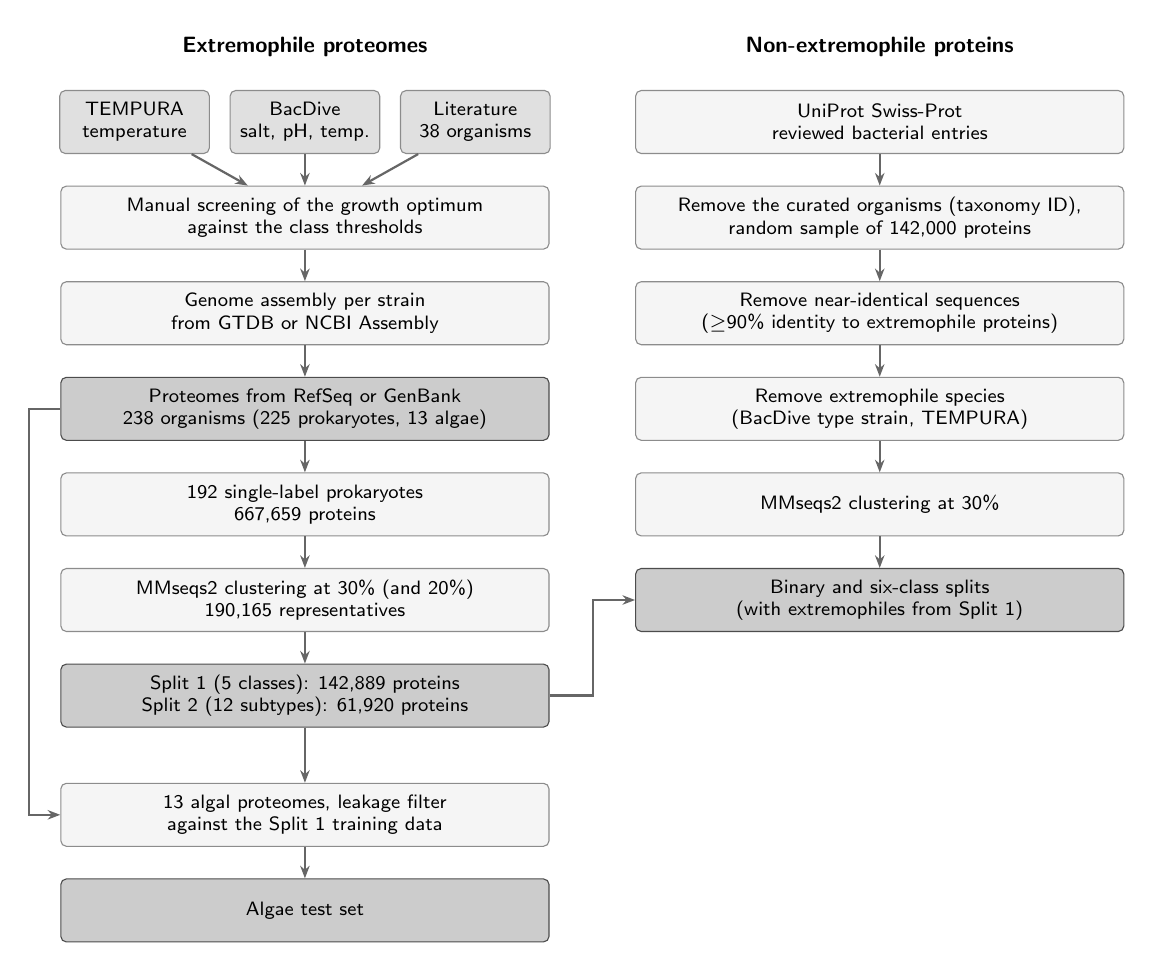
\begin{tikzpicture}[
    font=\sffamily\scriptsize,
    node distance=4mm and 3mm,
    box/.style={draw=black!45, rounded corners=2pt, fill=black!4, align=center, minimum width=62mm, minimum height=8mm},
    source/.style={box, fill=black!12, minimum width=19mm},
    result/.style={box, draw=black!70, fill=black!20},
    head/.style={font=\sffamily\footnotesize\bfseries},
    arrow/.style={-{Stealth[length=1.6mm]}, draw=black!60, thick},
]
% Extremophiles
\node[head] (h1) {Extremophile proteomes};
\node[source, below=3mm of h1] (bacdive) {BacDive\\salt, pH, temp.};
\node[source, left=2.5mm of bacdive] (tempura) {TEMPURA\\temperature};
\node[source, right=2.5mm of bacdive] (lit) {Literature\\38 organisms};
\node[box, below=of bacdive] (screen) {Manual screening of the growth optimum\\against the class thresholds};
\node[box, below=of screen] (genome) {Genome assembly per strain\\from GTDB or NCBI Assembly};
\node[result, below=of genome] (proteome) {Proteomes from RefSeq or GenBank\\238 organisms (225 prokaryotes, 13 algae)};
\node[box, below=of proteome] (single) {192 single-label prokaryotes\\667{,}659 proteins};
\node[box, below=of single] (cluster) {MMseqs2 clustering at 30\% (and 20\%)\\190{,}165 representatives};
\node[result, below=of cluster] (splits) {Split~1 (5 classes): 142{,}889 proteins\\Split~2 (12 subtypes): 61{,}920 proteins};
\node[box, below=7mm of splits] (algae) {13 algal proteomes, leakage filter\\against the Split~1 training data};
\node[result, below=of algae] (algaetest) {Algae test set};

% Non-extremophiles
\node[head] (h2) at ([xshift=73mm]h1) {Non-extremophile proteins};
\node[box, below=3mm of h2] (swiss) {UniProt Swiss-Prot\\reviewed bacterial entries};
\node[box, below=of swiss] (taxid) {Remove the curated organisms (taxonomy ID),\\random sample of 142{,}000 proteins};
\node[box, below=of taxid] (near) {Remove near-identical sequences\\($\geq$90\% identity to extremophile proteins)};
\node[box, below=of near] (species) {Remove extremophile species\\(BacDive type strain, TEMPURA)};
\node[box, below=of species] (ncluster) {MMseqs2 clustering at 30\%};
\node[result, below=of ncluster] (binary) {Binary and six-class splits\\(with extremophiles from Split~1)};

\foreach \a/\b in {tempura/screen, bacdive/screen, lit/screen, screen/genome, genome/proteome, proteome/single,
                   single/cluster, cluster/splits, splits/algae, algae/algaetest, swiss/taxid, taxid/near,
                   near/species, species/ncluster, ncluster/binary}
    \draw[arrow] (\a) -- (\b);
\draw[arrow] (splits.east) -- ++(5.5mm,0) |- (binary.west);
\draw[arrow] (proteome.west) -- ++(-4mm,0) |- (algae.west);
\end{tikzpicture}
